\section{Stratégies Probabiliste}

\subsection{Les différentes stratégies}
	
	\begin{frame}{Hasard}
		\begin{figure}
		    \centering
		    
\includegraphics[width=.5\linewidth]{images/TODO.png}
		    \caption{Algorithme Hasard Malin}
		    \label*{fig:algoHasardMalin}
		\end{figure}{}
	% Au hasard mais pas 2 fois sur la même case
	\end{frame}
	
	\begin{frame}{Chasse et Pêche}
	    \begin{figure}
		    \begin{subfigure}{.48\textwidth}
    		    \centering
    		    
\includegraphics[width=.9\linewidth]{images/TODO.png}
    		    % TODO : ajouter capture
                \caption*{Chasse et Pêche Mode Pêche}
                \label{fig:CPpeche}
            \end{subfigure}
            %\pause
            \begin{subfigure}{.48\textwidth}
                \centering
                
\includegraphics[width=.9\linewidth]{images/TODO.png} % TODO : ajouter capture
                 \caption*{Chasse et Pêche Mode Chasse}
                \label{fig:CPchasse}
            \end{subfigure}
        \end{figure}
    % Explications
	\end{frame}{}
	
	\begin{frame}{Chasse Pêche Croix}
		\begin{figure}
		    \centering
		    
\includegraphics[width=.5\linewidth]{images/TODO.png}
		    \caption*{Algorithme Chasse Pêche Croix}
		    \label{fig:CPC}
		\end{figure}{}
	% Idem CP mais seumement une case sur deux car bateaux de taille 2 ou plus
	\end{frame}
	
	\begin{frame}{Chasse Pêche Proba}
	    \begin{figure}
		    \begin{subfigure}{.32\textwidth}
    		    \centering
    		    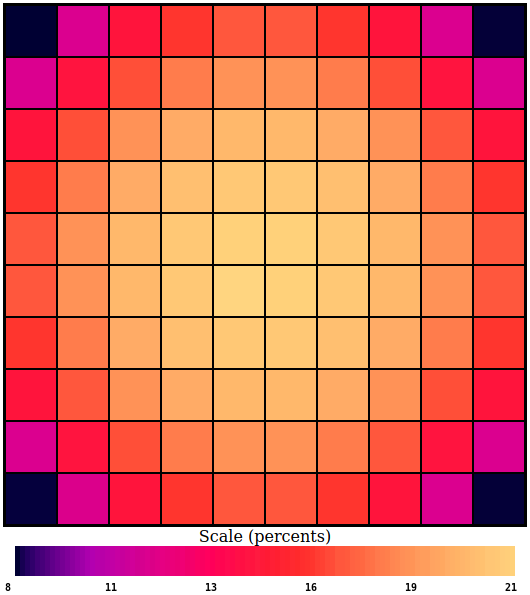
\includegraphics[width=.95\linewidth]{images/grille_initiale_proba.png}
                \caption*{Densité initiale}
                \label{fig:probaGrilleInit}
            \end{subfigure}
            %\pause
            \begin{subfigure}{.32\textwidth}
                \centering
                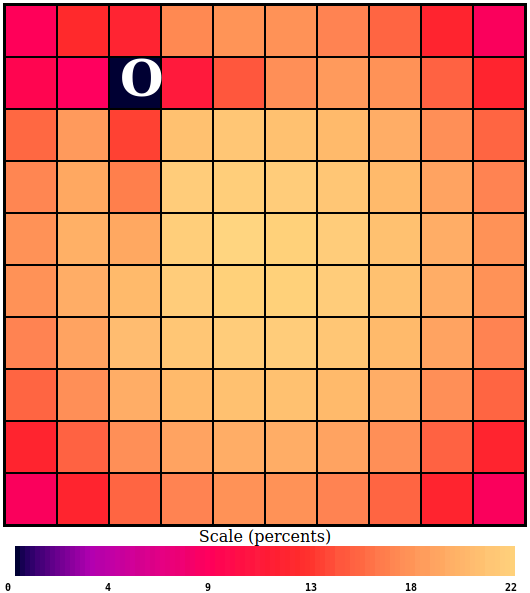
\includegraphics[width=.95\linewidth]{images/ploufC2.png}
                 \caption*{Plouf en C2}
                \label{fig:ploufC2}
            \end{subfigure}
            %\pause
            \begin{subfigure}{.32\textwidth}
                \centering
                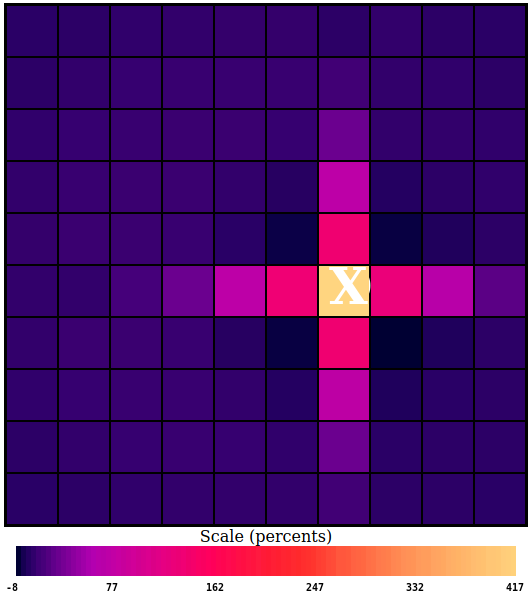
\includegraphics[width=.95\linewidth]{images/toucheG6.png}
                 \caption*{Touché en G6}
                \label{fig:toucheG6}
            \end{subfigure}
        \end{figure}
        \hfill Source : The Virtuosi
	\end{frame}{}
	
	\begin{frame}{Chasse Pêche Proba}
	    \begin{block}{Améliorations}
	        \begin{itemize}
	            \item Implémentation efficace : paradigme de programmation dynamique qui s'actualise en temps réel. Complexité en $\mathcal{O}(n\log{}n)$ %TODO : calculer la complexité
	            \item Prise en compte du nombre de bateaux et de leur taille
	            \item Mesure concrète de la qualité de l'algorithme
	        \end{itemize}
	    \end{block}
	\end{frame}{}
	
	\begin{frame}{Chasse Pêche Croix Proba}
	    \begin{block}{Algorithme Chasse Pêche Croix Proba}
	        \begin{itemize}
	            \item Algorithme perso
	            \item Mix entre CPC et CPP
	            \item Résultats médiocre 
	        \end{itemize}{}
	    \end{block}
	\end{frame}{}

\subsection{Résultats}
	
	\begin{frame}{Performances}
		\begin{figure}
		    \centering
		    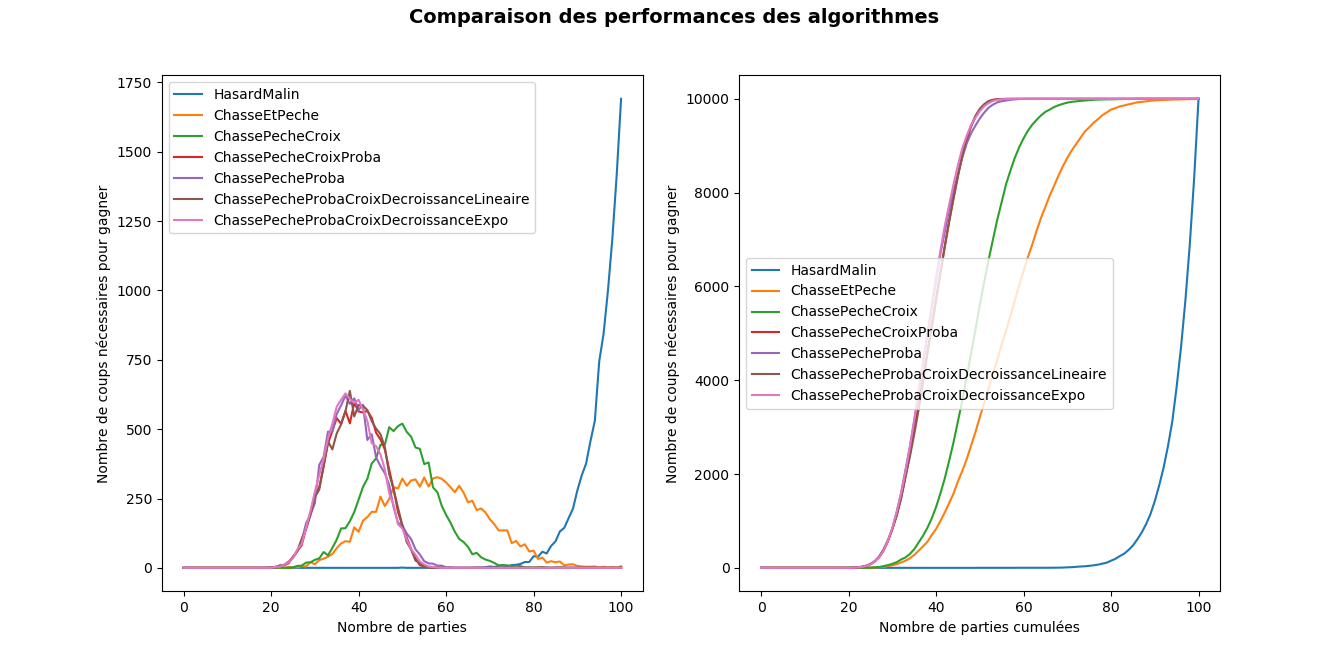
\includegraphics[width=.99\linewidth]{images/perfsstats.png}
		    \caption{Performances des différents algorithmes à stratégie probabiliste} % TODO : mettre les bons algos
		    \label{fig:perfsstats}
		\end{figure}{}
	\end{frame}